\documentclass[12pt]{article}
\usepackage{url,graphicx,tabularx,array}
\usepackage[margin=1in]{geometry}
\setlength{\parskip}{1ex} %--skip lines between paragraphs
\setlength{\parindent}{0pt} %--don't indent paragraphs

\usepackage{algorithmic}
\usepackage{algorithm}
\usepackage{ amssymb }
\usepackage{ latexsym }
\usepackage{ amsmath }
\usepackage{ amsthm }
%-- Commands for header
\renewcommand{\title}[1]{\textbf{#1}\\}
\renewcommand{\line}{\begin{tabularx}{\textwidth}{X>{\raggedleft}X}\hline\\\end{tabularx}\\[-0.5cm]}
\newcommand{\leftright}[2]{\begin{tabularx}{\textwidth}{X>{\raggedleft}X}#1%
& #2\\\end{tabularx}\\[-0.5cm]}

\newtheorem{defn}{Definition}[section]
\newtheorem{conjecture}{conjecture}[section]
\newtheorem{lemma}{Lemma}[section]
\newtheorem{corollary}{Corollary}[section]
\newtheorem{question}{Question}[section]
\newtheorem{proposition}{Proposition}[section]


%\linespread{2} %-- Uncomment for Double Space
\begin{document}

\title{Homework 4: CMPS 242}
\line
\leftright{\today}{Bryan Matsuo (bmatsuo@soe.ucsc.edu) \& John St. John (jstjohn@soe.ucsc.edu)} %-- left and right positions in the header
\begin{enumerate}
\item \textbf{Neural Networks:}
Here is the formula for the output at node 5 produced by the network from Figure 1 in the back-propagation handout. Note that the handout hints that the 0 node is often used to supply a learnable bias to the higher level nodes by having a constant z output value of 1. We used this definition of the 0 node.

\[
\sigma\left(w_{5,0}+w_{5,3}\sigma\left(w_{3,0}+\sum_{i=1}^2w_{3,i}z_i\right)+w_{5,4}\sigma\left(w_{4,0}+\sum_{i=1}^2w_{4,i}z_i\right) \right)
\]

\item \textbf{Decision Tree:}

Below are the impurity calculations given the choice of each node as root. The root with the lowest impurity is $x_1$ so that is the one that will be chosen.

Root=\[x_1: -\left(1/3\left(1\log_2 1 + 0\log_2 0 \right)+ 2/3 \left( 1/2\log_2 1/2 + 1/2\log_2 1/2\right)\right) = 0.667\]
Root=\[x_2: -\left(2/3\left( 2/3\log_2 2/3 + 1/3\log_2 1/3 \right) + 1/3 \left( 2/3\log_2 2/3 + 1/3\log_2 1/3 \right) \right)= 0.918 \]
Root=\[x_3: -\left(1/3\left( 2/3\log_2 2/3 + 1/3\log_2 1/3\right) + 2/3 \left( 2/3\log_2 2/3 + 1/3\log_2 1/3 \right)\right) =  0.918 \]


\item \textbf{Perceptrion Algorithm:}

\begin{enumerate}
\item \textit{Experiment 1:}

There is a definite relationship between both the number of gaps and the number of mistakes made. Figure~\ref{fig:gvm} clearly shows that the number of mistakes are upper bounded by $\frac{1}{\text{Gaps}^2}$, and decrease as the Gap size increases. Figure~\ref{fig:mvi} shows that the number of iterations required to reach a consistent hypothesis and the number of mistakes eventually made are highly correlated with eachother (Pearson's correlation coefficient of $0.9973$) so examining one variable against the Gap is equivalent to the other.



\item \textit{Experiment 2:}

We first generated two test sets, one with noisy labels and one noise-free
labels. These sets remained the same throughout this experiment.

We then generated 20 training sets of 100 examples each. For each training
set, the perceptron algorithm was trained once and evaluated against the
noisy test set and then separately trained and evaluated against the
noise-free test set.

For each training/test set combination we used the following set of prediction
rules to label the test instances.

\begin{enumerate}
    \item {\bf Last hypothesis}:
        Predict on ${\bf x}$ with $\text{sign}({\bf w}_{500} \cdot {\bf x})$.
    \item {\bf Voted hypothesis}:
        Predict on ${\bf x}$ with $\text{sign}\bigg(\sum_{t=1}^{500}\text{sign}({\bf w}_t \cdot {\bf x})\bigg)$.
    \item {\bf Longest survivor}:
        Predict on ${\bf x}$ with $\text{sign}({\bf w}_\ell \cdot {\bf x})$ where ${\bf w}_\ell$ is the longest surviving hypothesis from the 500 sampled training points.
    \item {\bf Voted Last 50}:
        Predict on ${\bf x}$ with $\text{sign}\bigg(\sum_{t=451}^{500}\text{sign}({\bf w}_t \cdot {\bf x})\bigg)$.
\end{enumerate}

Table~\ref{tab:ex2} shows number of mistakes seen by each prediction rule combined over all 20
training sets.

\begin{table}[htd]
\begin{center}
\begin{tabular}{l||c|c|c|c}
           & Last  & Voted Last 50 & Longest & Voted \\
               \hline
  noisy  &   286  &   282  &   980  &   290 \\ 
  noise-free  &    49  &    71  &   940   &   54 \\
\end{tabular}
\end{center}
\caption{
For each prediction rule, the total number of mistakes from predicting the
each test set (noisy and noise-free) of 100 points after training on each
the 20 randomly generated, noisy training sets. The number of mistakes is
out of 10000 predictions made for each pair of rule and test set.}
\label{tab:ex2}
\end{table}%


\begin{figure}[p]
\begin{center}
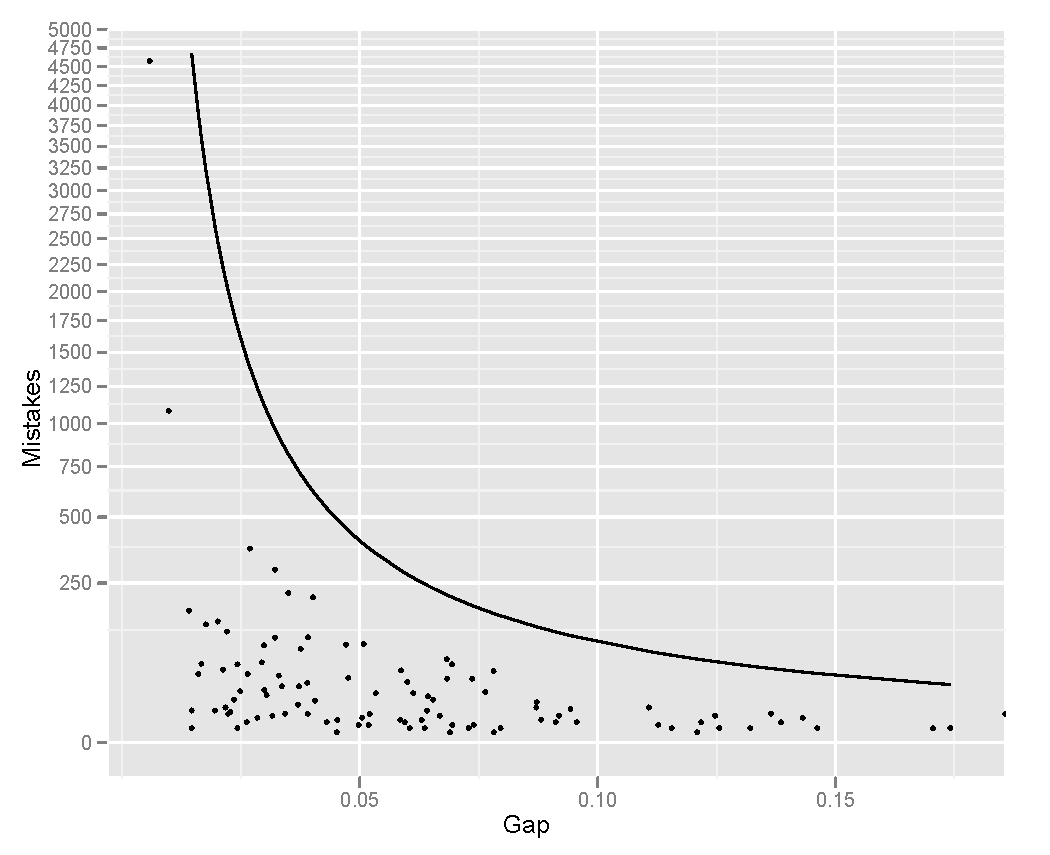
\includegraphics[scale=0.7]{ex1_gap_vs_Mistakes.pdf}
\caption{Comparing gaps to the total number of mistakes shows that as the gap increases in size, fewer mistakes are made. Interestingly, all of our points are well within the theoretical upper bound of the number of mistakes made is $\frac{1}{\text{Gap}^2}$}
\label{fig:gvm}
\end{center}

\end{figure}
\begin{figure}[p]
\begin{center}
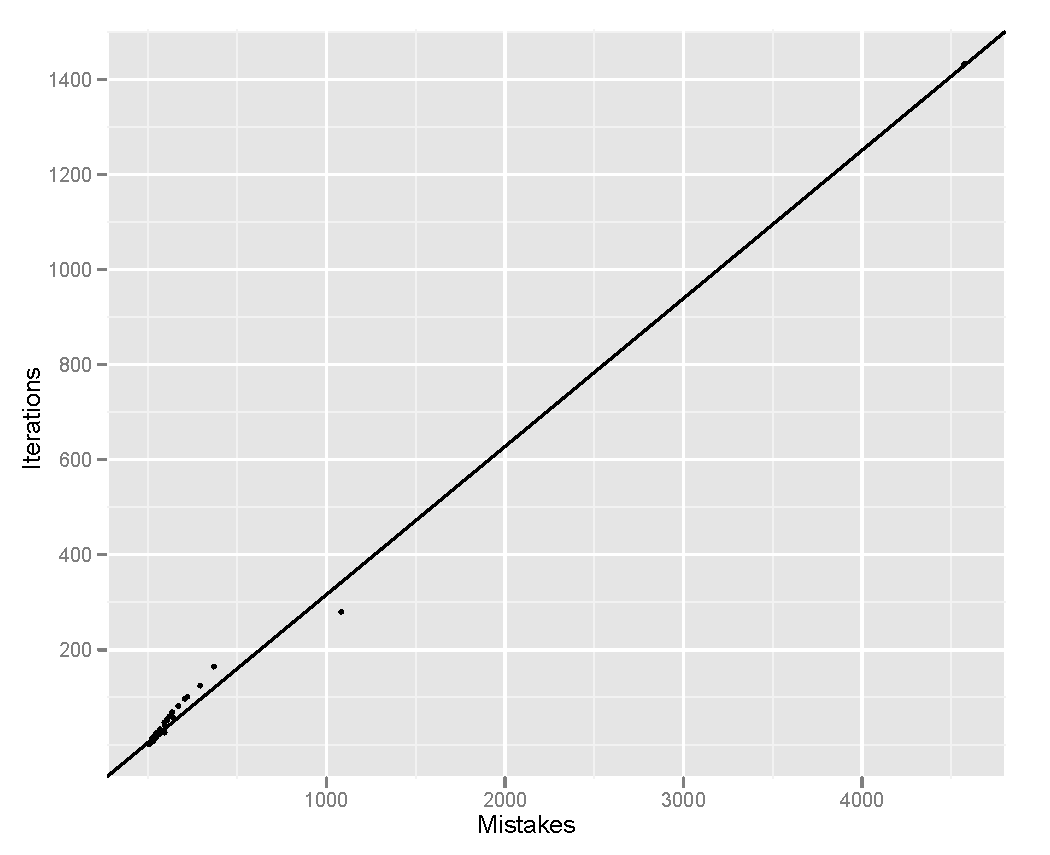
\includegraphics[scale=0.7]{ex1_iteration_mistakes.pdf}
\caption{Iterations and Mistakes are highly correlated with a Pearson's correlation coefficient of $0.9973$. Thus you are pretty safe just comparing one of those two values to the Gap as we did in Figure~\ref{fig:gvm}}
\label{fig:mvi}
\end{center}
\end{figure}

\end{enumerate}
\end{enumerate}
\end{document}
